% Neutral wrapper for drafting. Each section lives in sections/*.tex and contains no preamble material, so the same
% files can be \input by the thesis template or a journal class later. Packages used by the sections are listed here.
\documentclass[11pt]{article}
\usepackage[margin=25mm]{geometry}
\usepackage{amsmath,amssymb}
\usepackage{booktabs,tabularx,multirow}
\usepackage{graphicx}
% siunitx if installed (thesis template has it); minimal stand-ins otherwise
\IfFileExists{siunitx.sty}{\usepackage{siunitx}}{%
  \newcommand{\SI}[2]{##1\,##2}\newcommand{\num}[1]{##1}%
  \newcommand{\SIrange}[3]{##1--##2\,##3}}
\usepackage[colorlinks,allcolors=blue!50!black]{hyperref}
\usepackage{xcolor}
\graphicspath{{figures/}}
% drafting aids: remove for submission
\newcommand{\note}[1]{\textcolor{red!70!black}{[#1]}}
% notes block at the head of each section: what has to go in it (drafting only)
\newenvironment{notes}{\par\color{red!70!black}\small\noindent\textbf{Notes for this section}\begin{itemize}\setlength\itemsep{0pt}}{\end{itemize}\normalcolor\normalsize}

\title{Differentiable adaptive sensor placement for guided-wave thickness imaging:\\ from synthetic studies to laser-vibrometer data}
\author{draft}
\date{\today}

\begin{document}
\maketitle

% Section 1: Introduction.
\section{Introduction}\label{sec:intro}
\begin{notes}
\item Motivation: full-field LDV scans of plates give dense guided-wave data but are slow (here 6418 points, about 7\,h per shot); thickness imaging by full-waveform inversion (FWI) needs far fewer points if they are well placed.
\item Context: optimal experimental design (OED) for sensor placement in NDT/SHM and seismic imaging (greedy / D-, A-optimal selection, Bayesian OED); differentiable and adaptive design; scanning-LDV guided-wave imaging. Reviewer Xw48 (NeurIPS) asked for a comparison with greedy selection: we tried greedy log-det selection on the plate (failed, log items 30, 35--36) -- mention or put in the appendix.
\item Gap: adaptive, gradient-based sensor design has been shown on synthetic data; whether it helps on real laboratory data, with model error, is open.
\item This paper (thesis chapter, extension of the NeurIPS workshop paper): (1) the method and its cost (rematerialisation makes the design gradient fit one 11\,GB GPU); (2) a laboratory test on a PMMA plate with blind processing; (3) an honest account of where adaptivity helps: three comparisons from relaxed to strict.
\item Contributions list to finalise after the results of 24 Nov (case (i) with the random and offline controls; whether simulation design stays).
\item Outline of the paper (one sentence per section).
\item Contributions (25 Nov framing): (1) method and cost; (2) blind laboratory test on LDV data with model error; (3) the design places a movable array well (beats static and random), adaptively and without a prior model, matching a best-case advance plan; (4) an honest account from relaxed to strict comparisons, including where uniform coverage is as good.
\end{notes}

% Section 2: Method. Source: NeurIPS workshop paper (paper/main.tex), rewritten at journal length.
\section{Differentiable adaptive design}\label{sec:method}
\begin{notes}
\item Nested loop (F1): $K$ FWI updates on the current data, then one gradient step on the sensor positions; FWI first in the laboratory protocol (no design before data).
\item Three design objectives: oracle (needs the true model), waveform misfit (needs data at unmeasured points), stochastic illumination (needs neither). Illumination: $I(\mathbf x)$ = mean over sources and Rademacher probes $\mathbf q$ of $s^2$, $s = J^\top\mathbf q$ (per-source sensitivities), $3\times3$ smoothing; criterion $\mathrm{var}(I/\bar I) - \beta\log\bar I$, $\beta = 0.05$ (Eq.~\ref{eq:illumination}). Move Eq.~(6) of the workshop paper (illumination on the inherited model, constant in $\mathbf p$, low memory) to the main text (reviewer).
\item Second criterion used in the lab: $-\overline{\log(I+\varepsilon)}$ (define here or in Appendix A).
\item Positions as continuous variables, receivers sampled bilinearly; gradient through the forward solver by automatic differentiation (JAX).
\item Rematerialisation, 2--3 sentences, no figure: on the plate (620$\times$520 grid, 4 sources, 12--48 probes) the design gradient through all (source, probe) terms in one graph requested 142\,GB; wrapping each per-source term in a checkpoint (recomputed in the backward pass) brings it to about 3\,GB on one 11\,GB GPU, with identical gradients ($<10^{-5}$ relative). Enabler of the lab design, not a contribution on its own (log items 7, 11, 51).
\item Adam on positions: first step moves every coordinate by $\pm$lr (sign step) -- state it, it explains the 11.3\,mm first moves.
\end{notes}
% placeholder so that cross-references resolve while drafting
\begin{equation}
\Phi(\mathbf p) = \mathrm{var}\!\left(\frac{I(\mathbf x;\mathbf p)}{\bar I(\mathbf p)}\right) - \beta \log \bar I(\mathbf p)
\label{eq:illumination}
\end{equation}

\begin{figure}[ht]\centering
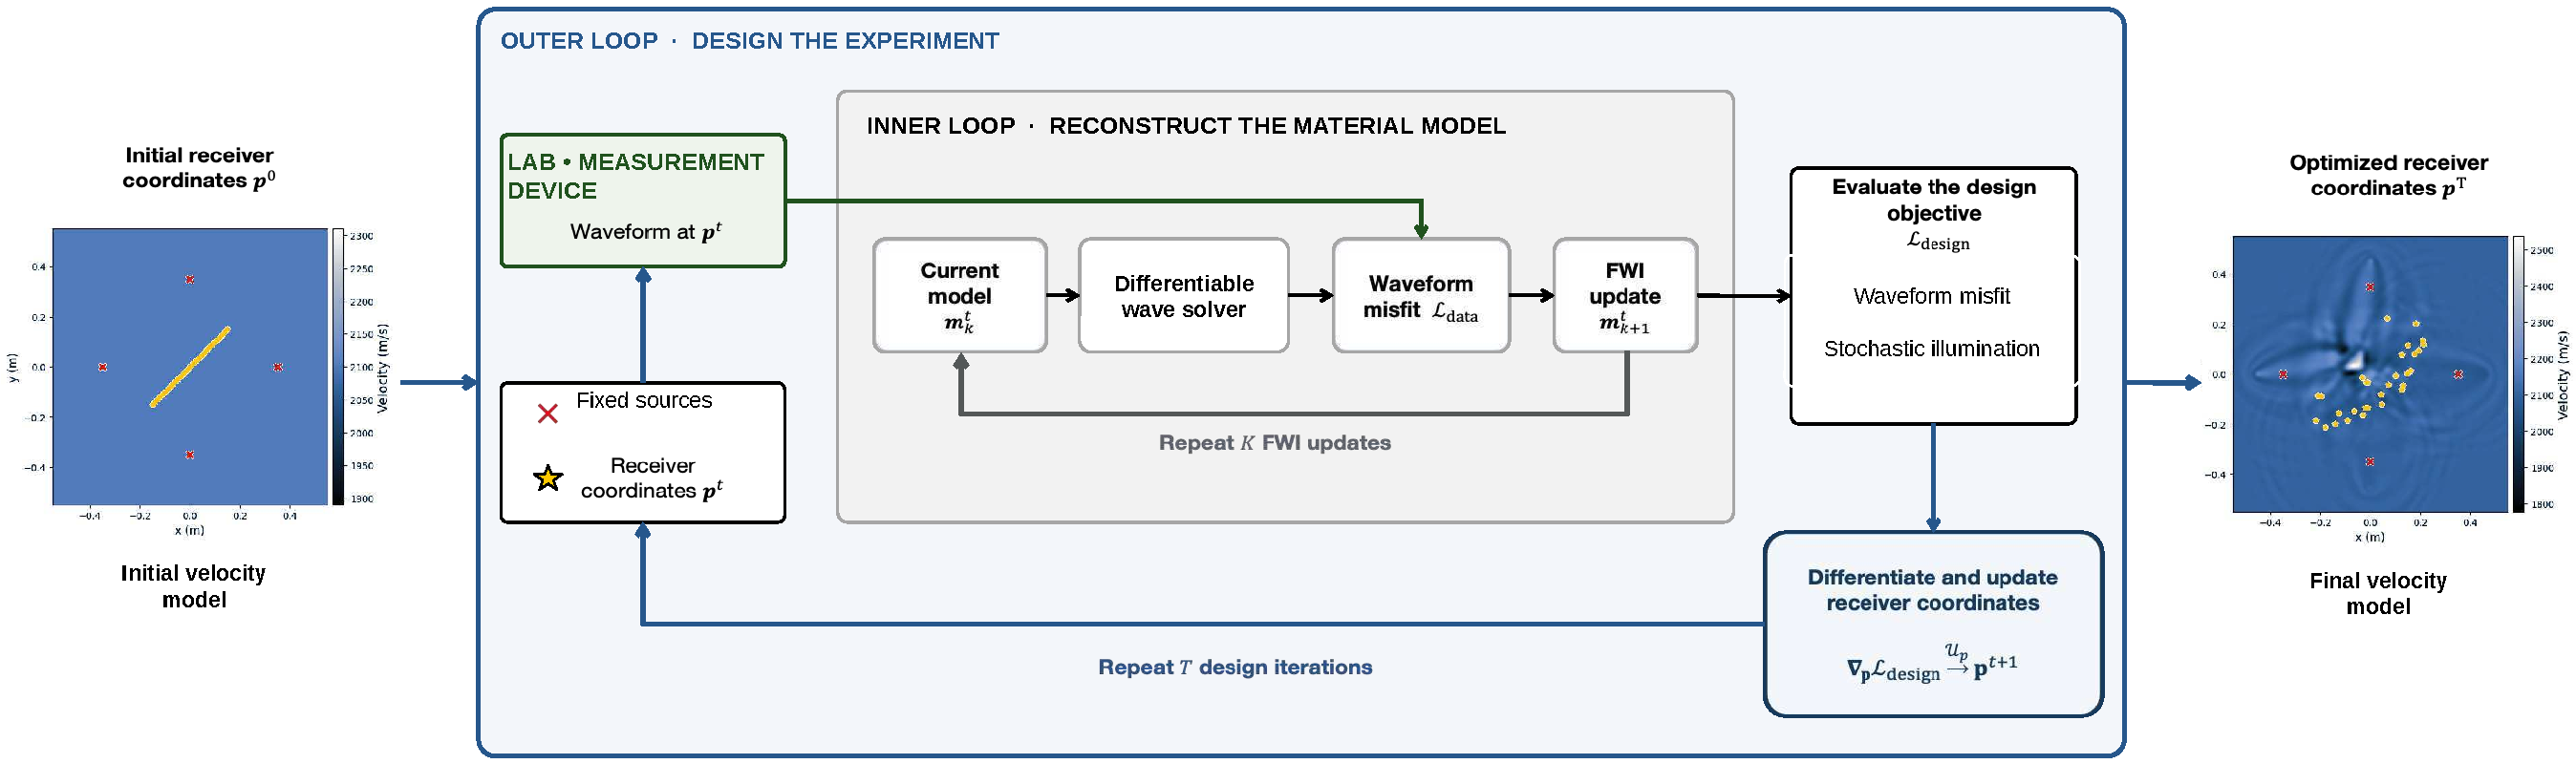
\includegraphics[width=\linewidth]{F1_loop.pdf}
\caption{\textbf{Concept.} Nested differentiable design loop (from the workshop paper), recoloured to the paper palette: measure at $\mathbf{p}^t$, $K$ FWI updates, evaluate the design objective, move the receivers along its gradient, measure again.}\label{fig:loop}
\end{figure}

% Section 3: Numerical study. Source: workshop results (oed_multiseed_full_autodiff_results), remat study (src/remat/README.md).
\section{Numerical study}\label{sec:numerical}
\begin{notes}
\item 2-D acoustic, 30 receivers, 10 seeds, fixed sensor count; improvement of the final model MSE over the fixed layout: oracle 18.6\,\%, illumination 16.7\,\%, waveform misfit 9.4\,\%, each in 10/10 seeds (F2). Illumination close to the oracle without true model or extra data: the objective taken to the lab.
\item Example run (F2b): true model, fixed-layout and designed reconstructions, receiver paths (MSE 3449 / 3024 / 3040 / 2668).
\item Cost figure and CPU/GPU benchmark dropped (25 Nov, user): the NeurIPS implementation did not use rematerialisation, so the comparison is not a result of this paper. Rematerialisation is described briefly in Sec.~\ref{sec:method}.
\item Reviewer points (NeurIPS) to address here: $\beta$ sweep, variance over seeds, scaling (answered by the lab plate: 620$\times$520 grid, real data).
\end{notes}
\begin{figure}[ht]\centering
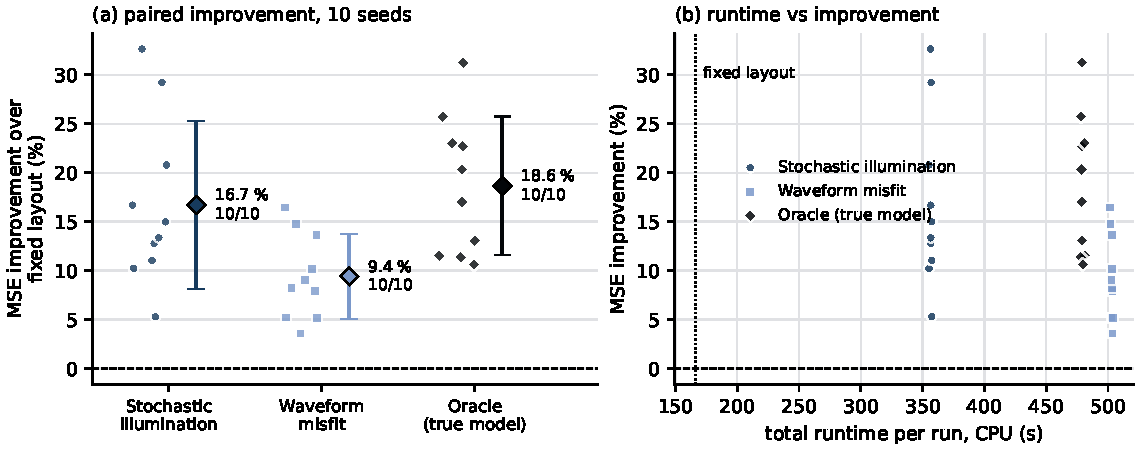
\includegraphics[width=\linewidth]{F2_numerical.pdf}\\[2mm]
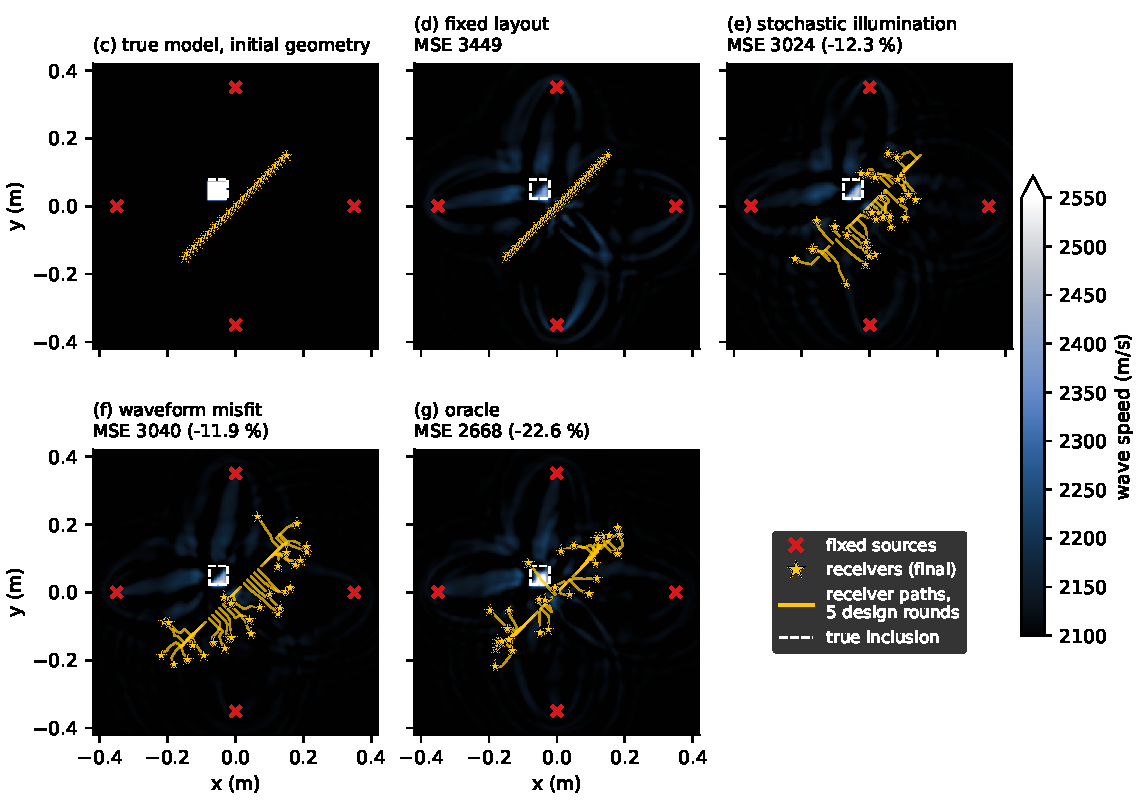
\includegraphics[width=0.85\linewidth]{F2b_numerical_maps.pdf}
\caption{\textbf{Numerical study} (2-D acoustic, 30 receivers, 10 seeds). (a) Paired improvement of the final model MSE over the fixed layout (illumination 16.7\,\%, waveform misfit 9.4\,\%, oracle 18.6\,\%, each 10/10); (b) the same against the total CPU runtime per run. (c--g) Example run: (c) true model with the fixed sources and the initial receiver line; (d) fixed-layout reconstruction; (e--g) reconstructions after 5 design rounds with the receiver paths, for illumination, waveform misfit and the oracle; MSE change relative to (d).}\label{fig:numerical}
\end{figure}


% Section 4: Laboratory experiment. Facts: ldv_processing_log.md items 0-2, step 1; figures F4, A1, A2.
\section{Laboratory experiment}\label{sec:experiment}
\begin{notes}
\item Specimen: PMMA plate $900\times835\times10$\,mm on foam pads; four PZT blocks $10\times10\times7$\,mm (5.3\,g) bonded on the back face; defects drilled from the back after the pristine scan: D1, D2 blind holes \O10\,mm, 6\,mm deep; D3 through-hole \O10\,mm; D4 blind hole \O8\,mm, 6\,mm deep; M1 steel cube 10\,mm glued on the back (F4, drawing A1).
\item Excitation: Ricker 40\,kHz; main mode A0 ($\lambda\approx25$\,mm, phase velocity $\approx1000$\,m/s); S0 visible at about 10\,\% of A0.
\item LDV: Polytec 3-D PSV on a robot (A2); $v_z$ used; fs 3.125\,MHz, 1.6\,ms, 20 averages, about 3.8\,s per point and shot.
\item Scans: pristine (6\,mm grid, 1650 points) and defect scan (3\,mm grid, 6418 points, about 7\,h per shot). The plate moved between the scans (registration on the direct waves: $T=(-3.6,-2.7)$\,mm), so the defect scan is inverted directly, without pristine subtraction.
\item Shots -- state neutrally: because of a fault in the excitation script, S1 is driven in every acquisition; the four shots are S1, S1+S2, S1+S3, S1+S4. The model simulates exactly the driven transducers of each shot. Two-shot set: S1 and S1+S3 (chosen as the farthest pair, without using the defects); one-shot set: S1+S3 only.
\item Pristine scan also had wrong-source points (independent clocks); the defect scan has none (timing fixed). Mention only as far as needed for the calibration (Sec.~\ref{sec:model}).
\item Preprocessing: band-pass 15--90\,kHz, resample 625\,kHz, window 400--1500\,\textmu s; dropouts (noise $>3\times$ median, about 10\,\%).
\item Every result-producing step is blind to the defects; their positions are used only for scoring.
\end{notes}
\begin{figure}[ht]\centering
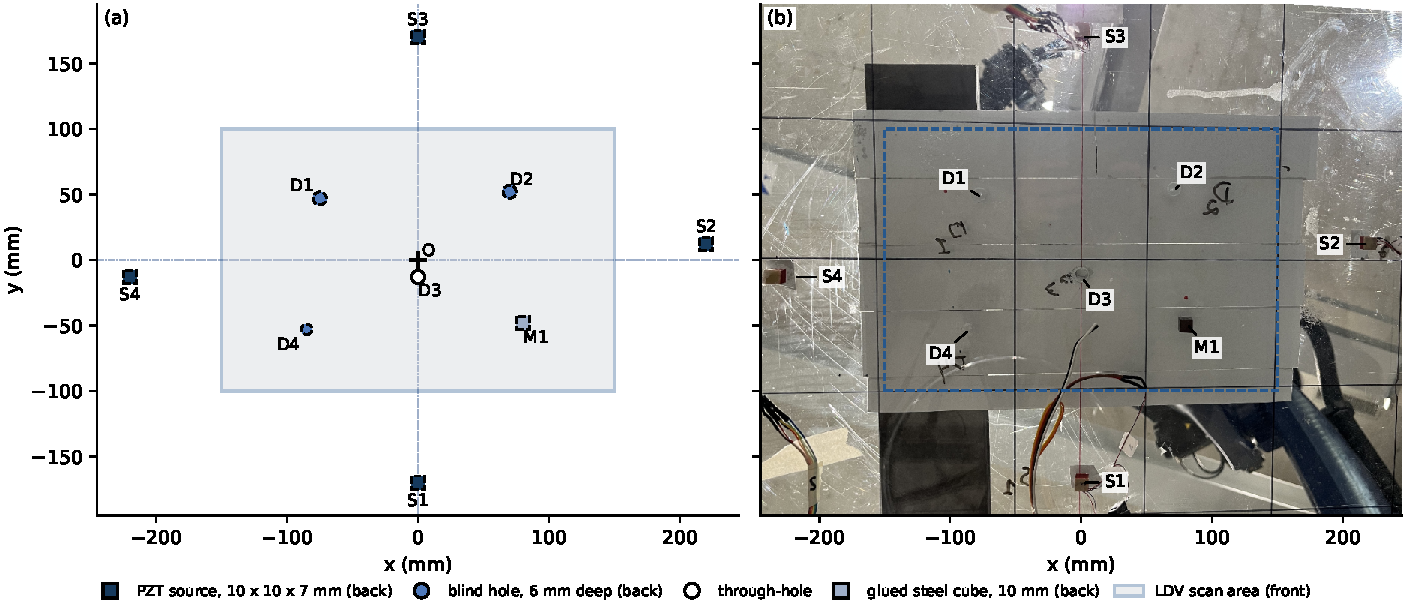
\includegraphics[width=\linewidth]{F4_specimen.pdf}
\caption{\textbf{Specimen.} (a) Front face (LDV side), positions from the scan centre O; (b) photo of the plate, top-down through the transparent PMMA, resampled into the same frame (homography on 9 control points, residuals $\le 2$\,mm) and annotated. Specimen: 10\,mm PMMA plate (900$\times$835\,mm), four PZT sources (10$\times$10$\times$7\,mm blocks, back face), blind holes D1, D2 (10\,mm) and D4 (8\,mm) 6\,mm deep from the back, through-hole D3 (10\,mm), glued steel cube M1 (10\,mm, back); dashed outlines = back face. Full drawing in Appendix Fig.~A1, laboratory setup in Fig.~A2.}\label{fig:specimen}
\end{figure}


% Section 5: Plate model, blind calibration and forward check. Facts: log steps 3, blind pipeline, items 65, 67; figure F3.
\section{Plate model and blind calibration}\label{sec:model}
\begin{notes}
\item Mindlin plate, 1\,mm finite-difference grid ($626\times518$), sponge (edges not modelled; window 450--800\,\textmu s ends before the edge echoes), mass-proportional damping (Q at 40\,kHz), vertical point forces, PZT blocks as added mass. Source signatures: one complex filter per frequency and transducer, re-estimated by variable projection.
\item Pristine calibration: velocity scale 0.995, Q 34.5, misfit 0.041 (0.028 in 450--650\,\textmu s), per-point correlation 0.98.
\item Blind self-calibration on the defect scan: robust IRLS weights, coordinate search on s, Q, source positions: s 0.990, Q 30; sources within 0.8\,mm of the oracle calibration and 1--5\,mm of the ruler. Down-weighted points sit at D3, M1, D1, D2 from the data alone. Table: s, Q, sources, misfit, correlation.
\item ``No surface'' points from amplitude (RMS $>1.5\times$ neighbour median): 17 of 6418, excluded.
\item Forward check (F3): pristine Mindlin 0.028 vs Salvus 3-D 0.037; defect scan: Mindlin pristine 0.082, Mindlin as built 0.076, Salvus as built 0.043, blind Mindlin inversion 0.042. Message: the plate model is adequate for the intact plate; its representation of the through-hole and the glued mass is the main model error.
\item Mindlin has no S0 (about 1\,\% of the energy): small part of the misfit.
\item Caveat: the background is calibrated on the full defect scan and used for every layout (same for all strategies, so comparisons are fair).
\end{notes}
\begin{figure}[ht]\centering
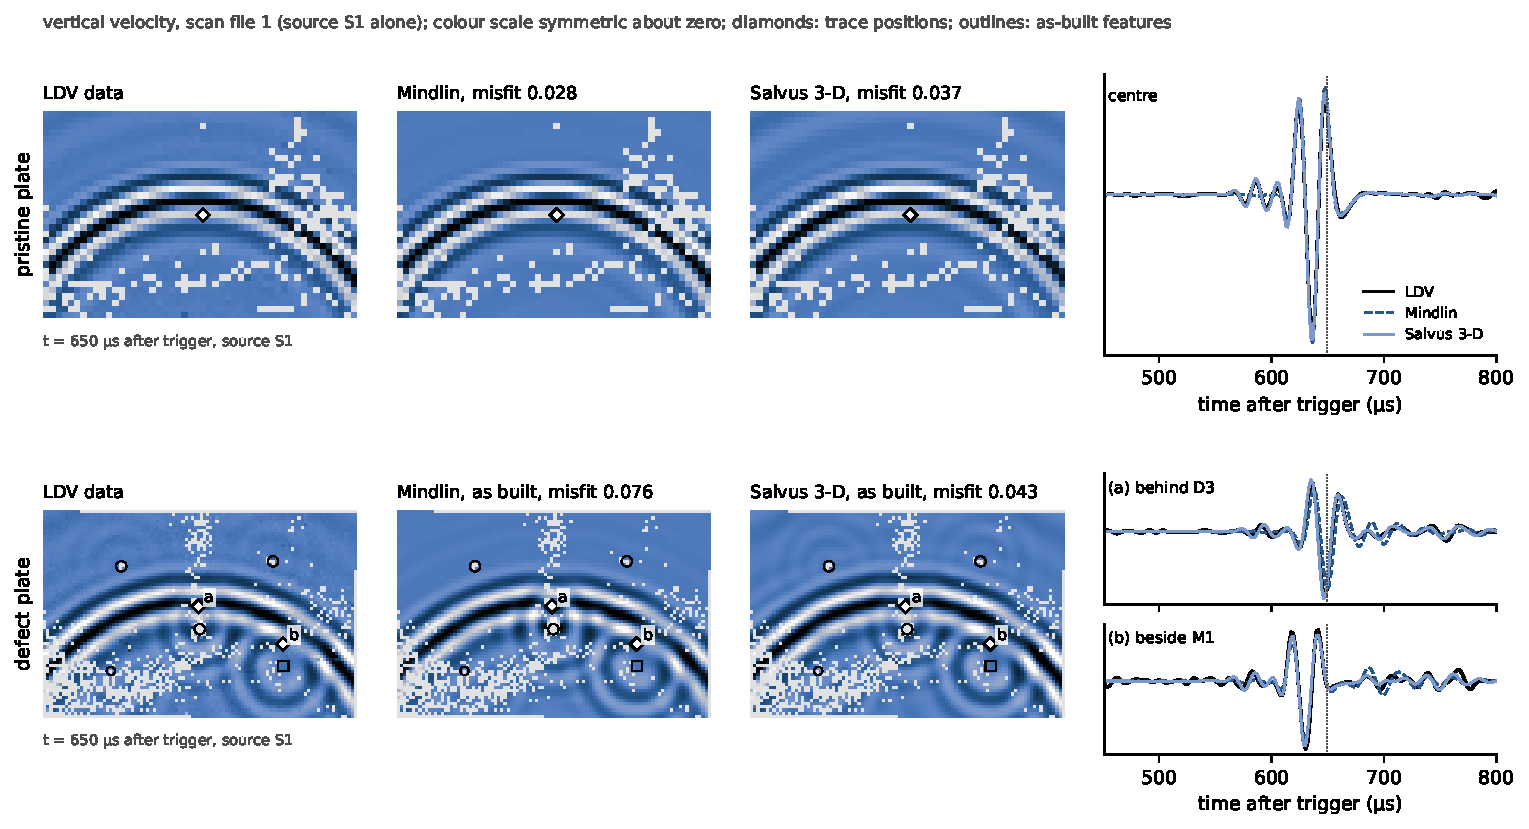
\includegraphics[width=\linewidth]{F3_waveforms.pdf}
\caption{\textbf{Forward-model check.} LDV vs Mindlin vs Salvus 3-D (full plate, free edges, PZT blocks, as-built holes and glued cube), same source-signature fit for every model; misfit over all files and points. Pristine plate: Mindlin 0.028 (calibrated on this scan), Salvus 0.037. Defect plate: Mindlin pristine 0.082, Mindlin as built (thinning, rigid cube) 0.076, Salvus as built 0.043, Mindlin blind inversion 0.042. The plate model is adequate for the intact plate; its representation of the through-hole and the glued mass is the weak point, which the blind inversion compensates with plugs.}\label{fig:forward}
\end{figure}


% Section 6: Full-scan inversion and scoring. Facts: log blind pipeline (v3 inversion), items 56-59, 89-92, 104-108; figure F7.
\section{Full-scan inversion and scoring}\label{sec:fullscan}
\begin{notes}
\item Inversion: thickness only, $h = h_{\min} + (\SI{10}{mm} - h_{\min})\,e^{m}$ with $h_{\min}=1$\,mm, mass follows $\rho h$; $m$ on a 3\,mm grid ($100\times66$) over the scan area, bilinear onto the 1\,mm grid; loss = mean over shots of the normalised residual energy + TV ($10^{-4}$); Adam, learning rate 0.03, 100 updates from the blind background (converged by 75--100). The cube is not in the model (unknown target).
\item Full-scan maps with 4, 2 and 1 shots (F7): all five features found; 29 / 34 / 3 false indications. The model renders M1 and D3 as stiff plugs with a thin ring (no void, no glued mass in a plate model).
\item Philosophy: an unmodelled feature must at least be located and contained.
\end{notes}
\begin{figure}[ht]\centering
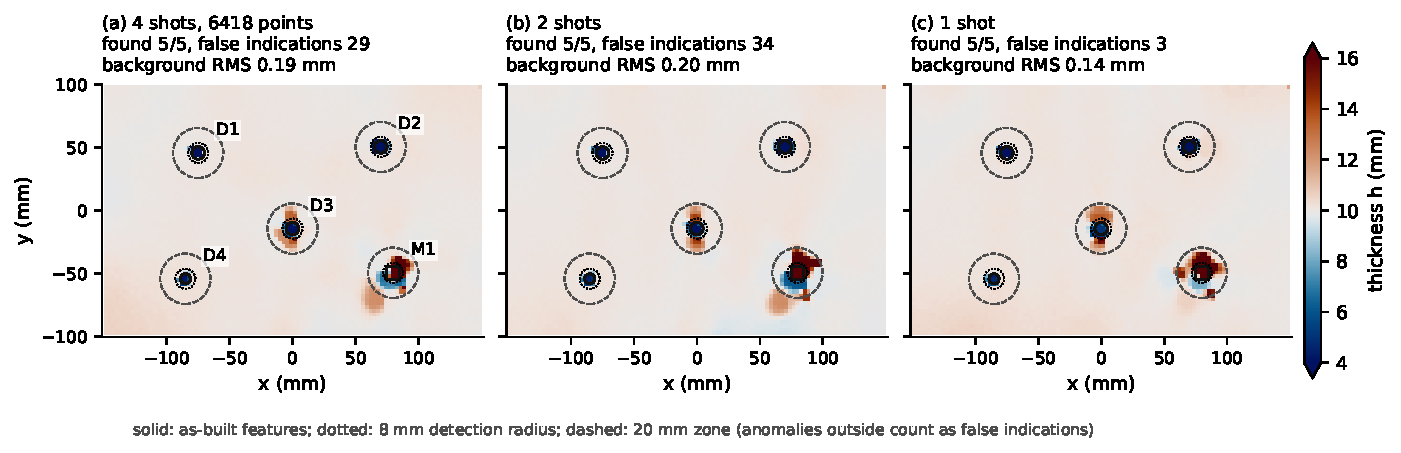
\includegraphics[width=\linewidth]{F7_fullscans.pdf}
\caption{\textbf{Blind full-scan inversions} with 4, 2 and 1 shots, and the scoring geometry (8\,mm detection radius, 20\,mm false-alarm zone). All five features are found in every case; the cube M1 and the through-hole D3 appear as stiff plugs with a thin ring.}\label{fig:fullscans}
\end{figure}


\subsection{Scoring}\label{sec:scoring}
\begin{notes}
\item Fixed-amplitude rule (pre-registered, internal name v3): anomaly $a=|h-\SI{10}{mm}|$; found if $a>3$\,mm within 8\,mm of the feature (all five, including M1); localisation error = distance to the peak of $a$ within 25\,mm; false indications = cells with $a>1$\,mm farther than 20\,mm (about half an A0 wavelength) from every feature, inside $|x|<140$, $|y|<90$\,mm; background RMS on the same cells; spill radius of M1 and D3. Ranking: found, then false indications, then background RMS. Term ``false indication'' (ASTM E1316).
\item Sensitivity (log items 90, 92): threshold 1.5--3\,mm and detection radius 4--20\,mm do not change the conclusions; say so in one sentence.
\item Fixed false-indication rate rule (exploratory): threshold of each map = 99th (95th) percentile of $a$ over the background cells, so every map has 1\,\% (5\,\%) false indications and methods differ only in detection (CFAR-type rule, common in NDT/radar). Motivation: sparse inversions underestimate amplitudes; D4 is often located correctly but below 3\,mm (log item 89).
\item \textbf{Defect-free-background argument}: in practice the background distribution would be obtained from a scan of a defect-free plate (or a defect-free region), inverted with the same layout and settings; here the cells more than 20\,mm from every feature play that role. State the limitation: a pristine-scan inversion may have a different background level than the damaged plate (scattered-field artefacts); a blind variant (whole-map percentile) weakens the 30-point results (log item 107) -- report in the appendix.
\item Why both rules are shown: the amplitude rule is pre-registered; the rate rule separates detection from amplitude calibration.
\end{notes}

\section{Sensor design on laser-vibrometer data}\label{sec:lab-design}
% Section 7.1: acquisition strategies of the laboratory design study (main text: concepts only; settings in Appendix A).
% Facts: reports/2026-11_specimen/ldv_processing_log.md (items 30-31, 39-40, 50, 55, 59-62, 81, 89, 93, 96, 104-115)
% and reports/2026-11_mssp_paper/notes/run_list.md. Figure: src/ldv_pmma/plot_strategies.py -> F11_strategies.

\subsection{Acquisition strategies}\label{sec:lab-protocols}

Every strategy is replayed on the dense scan of Section~\ref{sec:experiment}: when a strategy asks for a position, it
receives the recording of the nearest scanned point, and nothing else. All strategies thus draw on the same data and
differ only in where they measure and how they turn their measurements into a map. A layout of 30 points costs about
\SI{2}{min} of scanning per shot, against about \SI{7}{h} for the dense scan.

The strategies differ in three choices (Fig.~\ref{fig:strategies}).
\begin{description}
\item[What is limited.] Either the \emph{scan budget}: 30 points in total, measured at once or in three batches of
  ten. Or the \emph{number of sensors}: 30 sensors that are moved and measured at five successive positions, which
  amounts to about 145 measured positions. The first mode corresponds to a scan whose cost is the number of points;
  the second to an array with a fixed number of channels that can be repositioned, as in the numerical study.
\item[Who decides where to measure.] No design (regular, jittered or random layouts, or random moves); a design made
  \emph{before} measuring, on the defect-free background model; or an \emph{adaptive} design, made between
  measurements on the model inverted from the data so far, with the illumination criterion of
  Section~\ref{sec:method}.
\item[How the map is made.] In \emph{one pass}, with all data at once and 100 updates, as for the dense scan; or
  \emph{staged}, with the updates interleaved with the measurements. Adaptive designs need the staged form, because
  each design step uses an intermediate model; the total number of updates is 100 in both cases.
\end{description}

\begin{figure}[ht]\centering
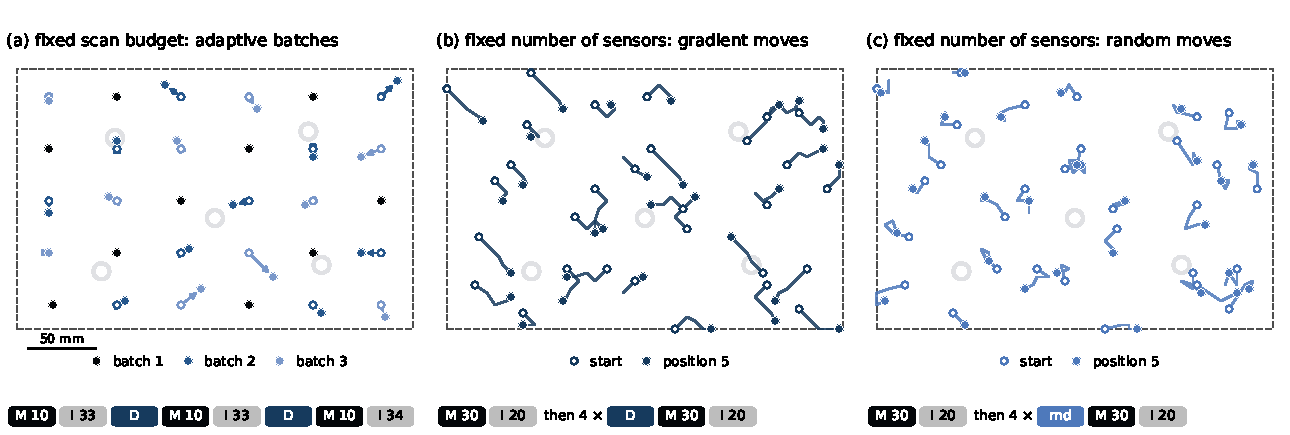
\includegraphics[width=\linewidth]{F11_strategies.pdf}
\caption{The two acquisition modes, drawn from three runs with four shots. (a) Fixed scan budget: 30 points in three
batches of ten; the first batch is measured as laid out, the next two are moved by the adaptive design (arrows, from the
planned to the measured position) on the model inverted from the batches before. (b) Fixed number of sensors: 30
sensors measured at five successive positions, each step following the illumination gradient on the current model.
(c) The same sensors and step lengths with random directions. Grey circles: the five features, for orientation only.
Bottom: sequence of measurements (M, number of points), inversion updates (I) and design steps (D) or random steps
(rnd).}\label{fig:strategies}
\end{figure}

Table~\ref{tab:strategies} places every strategy by the first two choices. Three further runs vary only the third:
\emph{progressive static} measures the static layouts in the same three batches with the staged inversion of the
adaptive batches; \emph{re-inversion} inverts the final 30 points of each adaptive run once, like a static layout; and
\emph{all visited positions} inverts the $\approx$145 positions of each moving array at once and compares them with a
static layout of the same size. All strategies are run with one, two and four shots from the same start layouts;
the settings are listed in Appendix~\ref{app:protocols}.

\begin{table}[ht]\centering\small
\caption{Strategies of the laboratory study, by what is limited and who places the points. Numbers: runs with four /
two / one shot.}\label{tab:strategies}
\begin{tabular}{@{}lll@{}}
\toprule
 & fixed scan budget (30 points) & fixed number of sensors (30 $\times$ 5 positions) \\ \midrule
no design            & static layouts \quad 8 / 7 / 7        & random moves \quad 3 / 5 / 5 \\
designed beforehand  & simulation design \quad 3 / 3 / 3 \note{24 Nov}  & offline moves \quad 3 / 5 / 5 \note{24 Nov} \\
adaptive             & adaptive batches \quad 5 / 5 / 4      & gradient moves \quad 3 / 5 / 5 \\
\bottomrule
\end{tabular}
\end{table}

The results are organised as three comparisons, from the most to the least permissive. In case (i), gradient moves
are compared with static layouts: the same number of sensors and the same inversion cost, but five times the scan.
In case (ii), adaptive batches re-inverted in one pass are compared with static layouts: the same scan cost, with
one extra inversion allowed. In case (iii), adaptive batches are compared with progressive static: the same scan and
the same inversion. Each step removes a possible source of advantage. In every case the controls with no design
(random moves, progressive static) and, where available, the designs made beforehand indicate how much of a
difference is due to adapting to the data.

Maps are scored with the two rules of Section~\ref{sec:scoring}: a fixed amplitude threshold, and detection at a
fixed false-indication rate. The comparison of gradient and random moves, and the tests of the adaptive batches
against static and progressive static layouts, were fixed before the runs they concern; the comparisons of cases (i)
and (ii) against static layouts and the fixed-rate rule were chosen after seeing results and are reported as
exploratory (Appendix~\ref{app:protocols}).

% Section 7.2: case (i), equal inversion cost. Facts: log items 59-62 (Q2 pairs), 104, 110-112; figures F8, F10a/b; results of run A and offline moves 24 Nov.
\subsection{Case (i): moving the sensors}\label{sec:case-i}
\begin{notes}
\item Pre-registered: gradient vs random moves, 13 pairs: gradient ranks higher in 10 of 13 (4 shots 3/3, 2 shots 4/5, 1 shot 3/5); 7 of 10 on the pairs specified in advance ($p=0.17$). With 4 shots only gradient moves find D4.
\item Against static 30 points (exploratory): mean found 5.00 / 4.40 / 4.20 vs 3.88 / 3.43 / 3.43 at 1\,\% rate (MWU $p=0.001$, paired 11/2/0); with the fixed-amplitude rule 5.00 / 4.20 / 3.40 ($p=0.021$, paired 8/4/1); random moves gain little ($p=0.18$ / 0.22): the gain comes from the direction, not the extra measurements.
\item Disclose: random moves have matched path lengths but smaller net displacement (13--14 vs 24--29\,mm).
\item Reference dense static scans (4 shots): regular 110 points 5/5, 26 false indications; the gradient array matches detection but not false indications (64--240).
\item \note{24 Nov}: all visited positions ($\approx$145) inverted at once vs static of the same size (mj, rg143); offline moves (designed on the background) vs gradient moves = value of adaptivity.
\item Figures: F10a row (i), F10b panel (i); sensor paths in Sec.~\ref{sec:paths}.
\item \textbf{24 Nov results}: moves planned beforehand (offline, best-case background model calibrated on the full defect scan) match gradient moves: same start 2/10/1 under every rule; 1\,\%: offline 4.67 / 4.40 / 4.20 vs gradient 5.00 / 4.40 / 4.20. Both beat random (offline vs random 7/5/1, $p=0.035$) and static 30 (11/2/0). Wording: the adaptive design matches a best-case design planned beforehand, without needing a prior model or design campaign.
\item Sweep geometry: designed moves keep their direction (cos 0.71--0.99) and end 23--35\,mm from their start; random moves wander (cos 0) and end 12--15\,mm away, at equal path length. A property of the design; direction vs distance not separated (disclose; no fixed-heading test).
\item Case (iv), $\approx$145 points, one-pass inversion on both sides: gradient-visited vs jittered static of the same size, v3 mean found 5.00 / 4.60 vs 4.33 / 4.80 (4 / 2 shots), all five at 4 shots 3/3 vs 1/3; false indications 66 / 137 vs 32 / 54; regular 143-point grid 5/5, 90 / 116. Competitive with uniform coverage, better on D4 at 4 shots, noisier background. At 1\,\% everything is at the ceiling.
\item F10a rows: (i) gradient, planned beforehand (blue), random (grey); (iv) gradient-visited and random-visited vs same-size static.
\end{notes}
\begin{figure}[ht]\centering
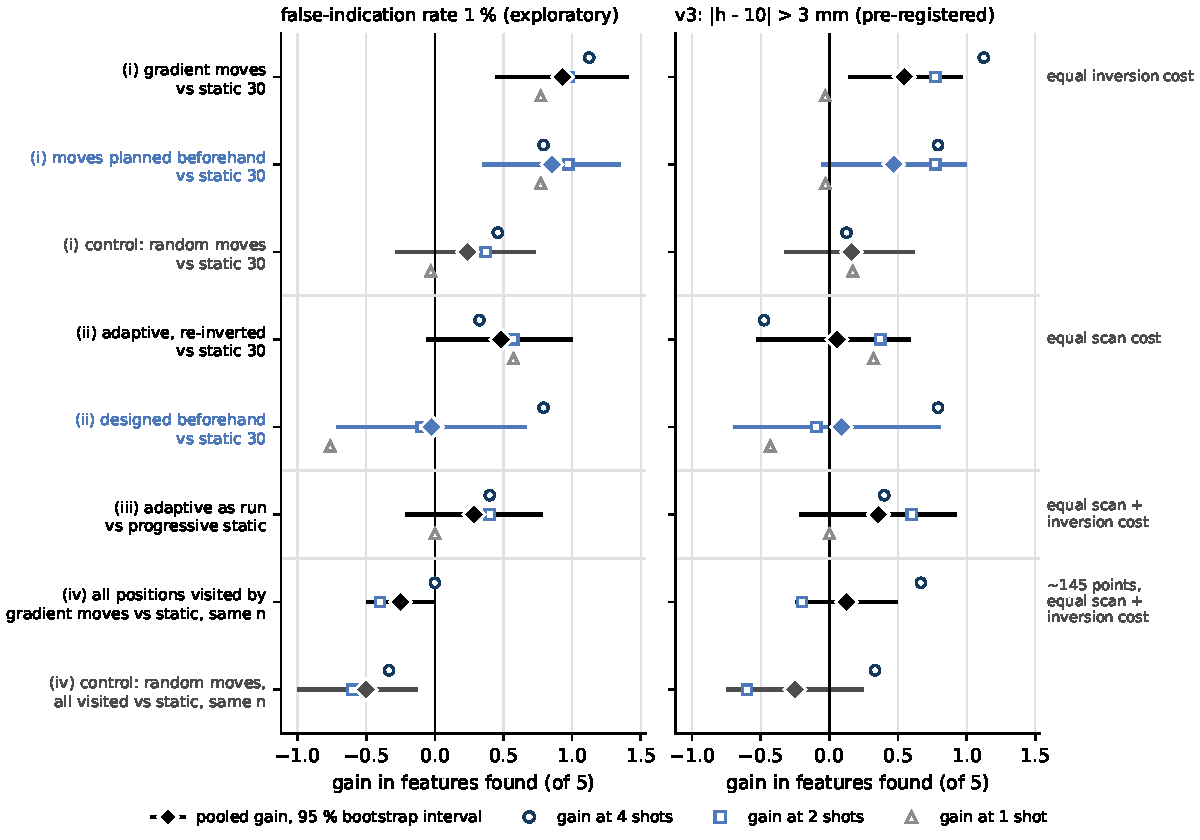
\includegraphics[width=0.8\linewidth]{F10a_funnel.pdf}
\caption{\textbf{Where the design helps: from relaxed to strict} (exploratory). Gain in features found (of 5) of the designed variant over its baseline; diamonds: pooled gain with 95\,\% bootstrap interval; open markers: gain at 4, 2 and 1 shots. Left: fixed 1\,\% false-indication rate; right: v3 (pre-registered). (i) equal inversion cost: 30 sensors moved along the illumination gradient vs static 30 points; blue: the same moves planned beforehand on a best-case model (calibrated on the full defect scan); grey: random moves. (ii) equal scan cost: adaptive points re-inverted in one pass; blue: 30 points designed beforehand. (iii) equal scan and inversion cost. (iv) about 145 points: all positions visited by the moving arrays, inverted in one pass, vs a static layout of the same size (4 and 2 shots).}\label{fig:funnel}
\end{figure}

\begin{figure}[ht]\centering
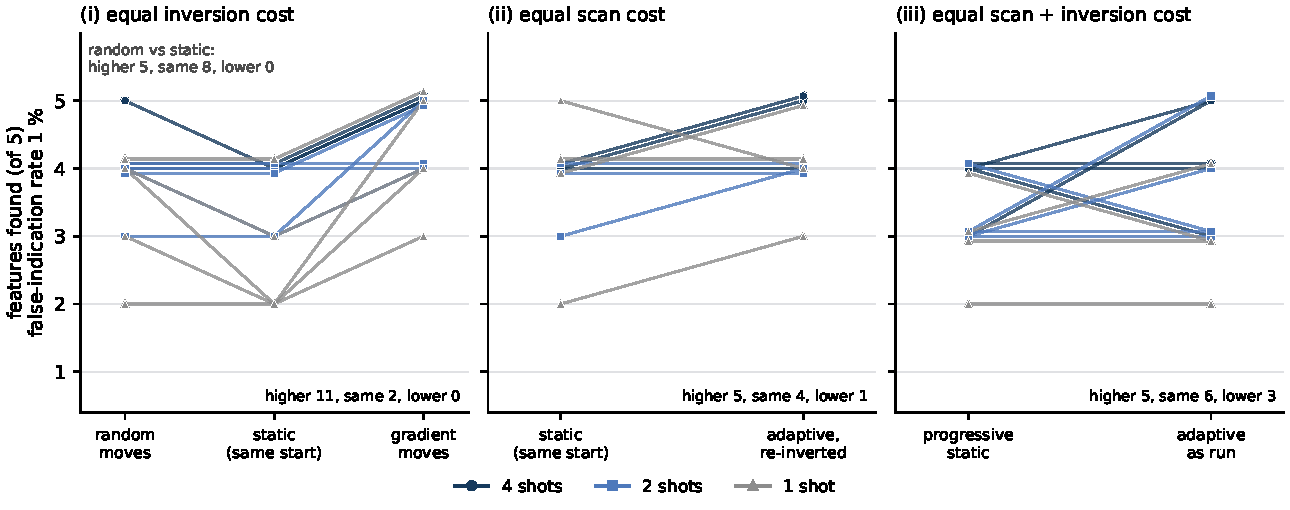
\includegraphics[width=\linewidth]{F10b_slopes.pdf}
\caption{\textbf{Paired view of Fig.~\ref{fig:funnel}} (1\,\% false-indication rate). Each line is one start layout, from its baseline to its designed variant; counts of start layouts that find more, the same or fewer features.}\label{fig:slopes}
\end{figure}


% Section 7.3: case (ii), equal scan cost. Facts: log items 88-89, 94-95, 103, 108; figures F8c/F8d, F10a.
\subsection{Case (ii): the same scan budget}\label{sec:case-ii}
\begin{notes}
\item Pre-registered Fisher test (all five found, adaptive batches vs static): 2/5 vs 1/8, 1/5 vs 0/7, 0/4 vs 1/7 -- not significant.
\item Diagnosis: D4 is located correctly by the adaptive runs but too weak (1.4--2.5\,mm); the round-2 designs chase false thin spots of the 20-point model.
\item Re-inversion (adaptive points, one pass) vs static at 1\,\% rate (exploratory): 4.20 / 4.00 / 4.00 vs 3.88 / 3.43 / 3.43, all five 4/14 vs 2/22, MWU $p=0.022$; paired with the same start 5/4/1 ($p=0.11$); fixed-amplitude rule: no gain. False indications lower than as run in 12 of 14 re-inversions.
\item Second criterion ($-\overline{\log I}$): no gain anywhere (report, do not hide).
\item \note{24 Nov}: simulation design (designed beforehand) vs static and vs re-inverted adaptive: if it is as good, the gain is from design, not adaptivity. Decide whether to keep.
\item \textbf{24 Nov results}: 30 points designed beforehand (3 per shot): 1\,\% 4.67 / 3.33 / 2.67, v3 4.67 / 3.33 / 3.00 vs static 3.88 / 3.43 / 3.43: no gain except with 4 shots (same start 3/2/4). Re-inverted adaptive vs designed beforehand, same start: 4/4/1 (1\,\%), 5/3/1 (5\,\%, $p=0.11$), 2/4/3 (v3): a small point for designing with the data.
\item Second criterion: move to the appendix (no gain anywhere).
\end{notes}

% Section 7.4: case (iii), equal scan and inversion cost. Facts: log items 96-98, 103, 109.
\subsection{Case (iii): the same scan and the same inversion}\label{sec:case-iii}
\begin{notes}
\item Adaptive batches vs progressive static (same batches, same 33/33/34 inversion, no design); pre-registered paired sign test (found, then false indications): 7 of 14, $p=0.61$.
\item On features found alone: higher at 4 and 2 shots under both rules (e.g. 1\,\%: 4.20 vs 3.80, 3.60 vs 3.20), equal at 1 shot; all five 3/14 vs 0/14; not significant (MWU $p$ 0.13--0.21). Adaptive runs have more false indications under the amplitude rule (median 292 vs 232 at 4 shots).
\item Re-inversion beats progressive static clearly (10/3/1 at 1\,\%): the staged inversion costs about as much as the design gains.
\item Second criterion: no gain.
\end{notes}

% Section 7.5: where the sensors go. Figures F9, F9b, F9c; log items 56, 60, 89.
\subsection{Where the sensors go}\label{sec:paths}
\begin{notes}
\item Sensor paths over the final maps (F9: 4 shots, j30a start; F9b 2 shots, x48c; F9c 1 shot, j30b): gradient-moved sensors sweep straight lines (cosine between consecutive moves 0.52--0.75), random ones wander (about 0).
\item The design is not attracted to the unmodelled cube (share of points within 30\,mm of M1 similar to the whole scan).
\item D4: detection does not follow the distance to the nearest point nor the number of source--receiver paths (log item 89): illumination, not proximity.
\item Two- and one-shot paths: Figs.~\ref{fig:paths-2} and \ref{fig:paths-1} (Appendix~\ref{app:figures}).
\item Possibly merge into 7.2 if space is short.
\end{notes}
\begin{figure}[ht]\centering
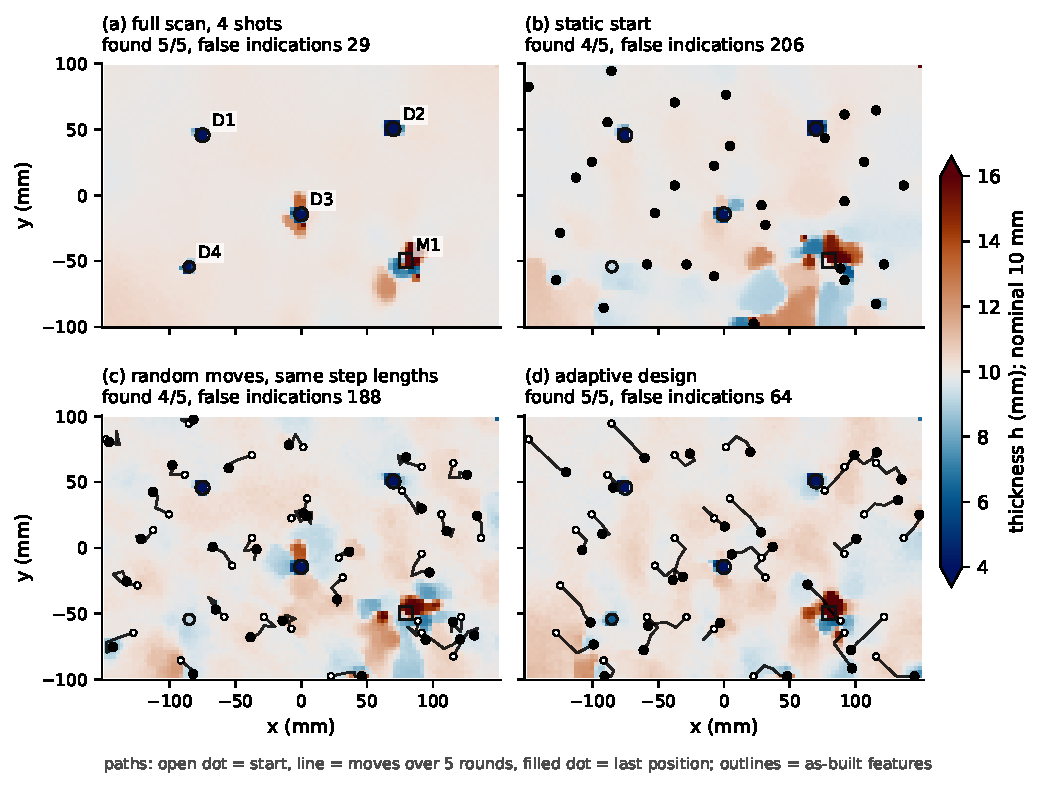
\includegraphics[width=0.9\linewidth]{F9_paths_ad_j30a.pdf}
\caption{\textbf{Where the sensors go, 4 shots} (best adaptive run, j30a start). (a) full scan, (b) static start, (c) random moves, (d) adaptive design. Adaptive sensors sweep straight lines and find D4; random moves stay near their start.}\label{fig:paths}
\end{figure}


% Section 8: Discussion.
\section{Discussion}\label{sec:discussion}
\begin{notes}
\item Where adaptivity helps: strongest when the number of sensors is limited and they can be moved (case (i)); weaker at a fixed scan budget, and not significant once scan and inversion are matched (case (iii)). Depends on the 24 Nov controls (offline moves, simulation design).
\item The staged inversion: needed by adaptive design, costs detection; re-inverting at the end recovers it.
\item Scoring: amplitude vs fixed false-indication rate; defect-free reference scan in practice.
\item Model error: through-hole and glued mass as plugs; containment of unmodelled features is the open weakness of sparse layouts (spill 19--45\,mm vs 10--16\,mm for full scans).
\item Limitations: one specimen, five features, D4 drives most differences; replay instead of a live closed loop; no S0, edges not modelled, $v_z$ only; background calibrated on the full scan; random-move net-displacement confound; multiple exploratory views (state them).
\item Practical reading: a dense regular scan of about 110 points already recovers everything on this plate; adaptivity is for settings where measurements or channels are expensive (contact sensors, robot-mounted arrays).
\item Transfer to metal plates / other specimens; live closed loop as next step.
\item \textbf{Framing (25 Nov)}: the design criterion is what places sensors well; running it adaptively reaches the result of a best-case advance plan without one. Planning beforehand needs a calibrated model of each specimen and geometry and a design run per setup; our offline control had a model calibrated on the full defect scan.
\item Irregular geometries (curved edges, stiffeners, cut-outs, areas the laser cannot reach): a regular grid may not fit; an illumination-based adaptive design may have an edge there. Untested (rectangular scan area); future work.
\item Dense uniform scans are the honest ceiling when scanning is cheap: at $\approx$145 points a uniform layout is as good for detection with a cleaner background.
\end{notes}

% Section 9: Conclusion.
\section{Conclusion}\label{sec:conclusion}
\begin{notes}
\item Three to five sentences: method and cost; lab result as the three cases; the take-home on where adaptivity helps; the open problem (criteria and models that contain unmodelled features).
\end{notes}


\appendix
% Appendix A: settings of the acquisition strategies and statistics (details moved out of Section 7.1).
% Facts: ldv_processing_log.md items 30-31, 39-40, 50, 55, 60-61, 81, 89, 93, 96, 104-114.

\section{Settings of the laboratory study}\label{app:protocols}

\paragraph{Replay.} A requested position is snapped to the nearest scanned point not yet taken in the same round
(at most \SI{3}{mm} away on the \SI{3}{mm} scan grid). Points flagged as dropouts or ``no surface''
(Section~\ref{sec:model}) are unusable in the replay as in the dense scan. The time needed to reposition the laser
heads is not included; it is small compared with the averaging time per point (about \SI{3.8}{s} per point and shot).

\paragraph{Start layouts.} Thirty points on the scan area: a cell-centred $6\times5$ regular grid; jittered layouts
with one random point in each cell of the $6\times5$ grid (seeds a--d); random layouts of 30--31 points (seeds a--d);
and, with four shots, a corner-anchored regular grid of \SI{48}{mm} spacing. With one shot some points of the
two-shot start layouts are dropouts, which leaves 24--31 usable points; the strategies compared on such a start use
the same points.

\begin{table}[ht]\centering\small
\caption{Settings of the strategies. Probes: Rademacher vectors per evaluation of the illumination criterion.}
\label{tab:settings}
\begin{tabularx}{\linewidth}{@{}l X X X@{}}
\toprule
 & adaptive batches & gradient / random moves & designed beforehand \\ \midrule
points or sensors & 30 in 3 batches of 10, cell $(c_x,c_y)\mapsto$ batch $(c_x+2c_y)\bmod 3$ & 30 sensors, 5 positions (4 moves) & 30 (simulation design); 30 sensors (offline moves) \\
design model & current inversion & current inversion (random: none) & defect-free background \\
design steps & 20 Adam steps of \SI{1.5}{mm} per batch, measured points fixed & 1 Adam step of \SI{8}{mm} per move, optimiser state carried & 60 Adam steps of \SI{1.5}{mm} (simulation); as moving array (offline) \\
probes & 12, redrawn every step & 48 & 12 (simulation); 48 (offline) \\
validation & every 10 steps, snapped layout on 4 separate probe sets, best kept & none & as adaptive batches (simulation) \\
inversion & staged 33 / 33 / 34 updates on all points so far & 5 $\times$ 20 updates on the current 30 positions, warm start & one pass, 100 (simulation); as moving array (offline) \\
\bottomrule
\end{tabularx}
\end{table}

\paragraph{Random moves.} Each sensor moves in every round by the same distance as its partner in the gradient run
from the same start, in a direction drawn uniformly at random. Path lengths are matched; net displacements are not,
because gradient moves keep their direction from round to round (Adam momentum): after four moves gradient-moved
sensors are \SIrange{24}{29}{mm} from their start, randomly moved ones \SIrange{13}{14}{mm}. Part of a gain of the
gradient moves may therefore come from covering more ground.

\paragraph{Larger budget.} \emph{All visited positions}: the 116--153 distinct positions of each moving array
inverted once (100 updates), against a jittered layout with exactly the same number of points (one cell per point
on the smallest $n_x\times n_y$ grid of aspect $6{:}5$, surplus cells dropped at random) and a cell-centred
$13\times11$ regular grid (143 points). Random-move arrays visit 1--9 fewer distinct positions than their gradient
partners, because some positions are measured twice.

\paragraph{Second criterion.} $-\overline{\log(I+\varepsilon)}$ with $\varepsilon=10^{-3}\,\bar I$ (uniformity in which
bright spots saturate, plus the overall illumination at unit weight, i.e.\ diagonal D-optimality), run as adaptive
batches from the jittered starts with one, two and four shots, each followed by its re-inversion.

\paragraph{Statistics.} Paired comparisons use one-sided sign tests over start layouts, ranking runs by features
found, then false indications, then background RMS (ties dropped). Group comparisons use a one-sided Fisher test on the
share of runs that find all five features and a one-sided Mann--Whitney test on the number found, centred on the
baseline mean of each shot setting so that shot settings can be pooled. Pooled gains are averages of the per-shot
differences of means, weighted by the number of designed runs, with 95\,\% bootstrap intervals (runs resampled within
each group and shot setting, 5000 draws).

\paragraph{What was fixed in advance.} Before the runs they concern: the gradient-versus-random comparison of the
moving arrays (sign test; the scoring rule of Section~\ref{sec:scoring} was fixed after the first three of the 13
pairs had run, so 10 pairs are fully pre-specified); the Fisher test of the adaptive batches against the static
layouts; the same test for the re-inversions and for the second criterion; and the paired test of the adaptive
batches against progressive static. Chosen after seeing results: detection at a fixed false-indication rate, the
comparisons of cases (i) and (ii) against static layouts, the bootstrap intervals and the larger-budget and offline
checks. No correction for multiple comparisons is applied; $p$-values of the exploratory analyses are descriptive.

% Appendix B: figures not (yet) in the main text, for review. Captions from the archived outline.
\section{Additional figures}\label{app:figures}
\begin{notes}
\item Sensor paths with two and one shot (companions of Fig.~\ref{fig:paths}), specimen drawing, setup photo.
\item Removed from the paper 25 Nov (files kept in figures/): the 13 gradient/random pairs (F8\_pairs), and the fixed-budget figures F8b (matched budget), F8c (detection curves), F8d (fixed rate); their content is in Figs.~\ref{fig:funnel} and \ref{fig:slopes}.
\end{notes}


\begin{figure}[ht]\centering
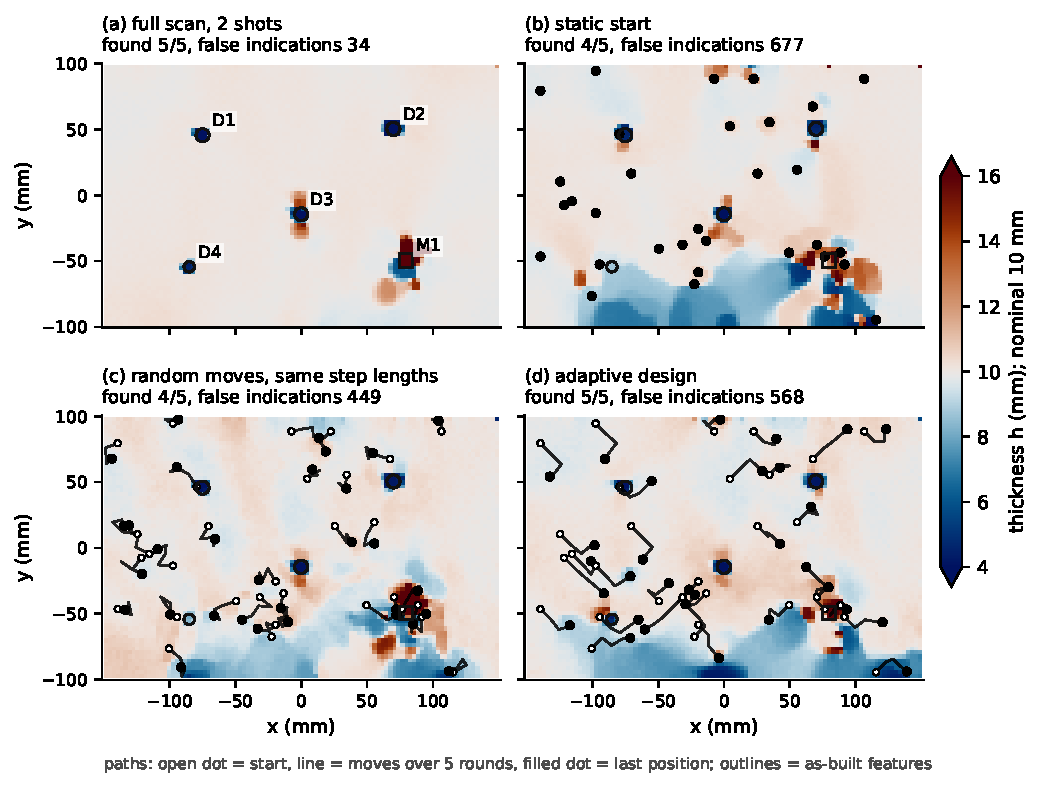
\includegraphics[width=0.9\linewidth]{F9_paths_a2_x48c.pdf}
\caption{\textbf{2 shots} (best adaptive run, x48c start): all five features found, but a thin band along the lower edge (568 false indications).}\label{fig:paths-2}
\end{figure}

\begin{figure}[ht]\centering
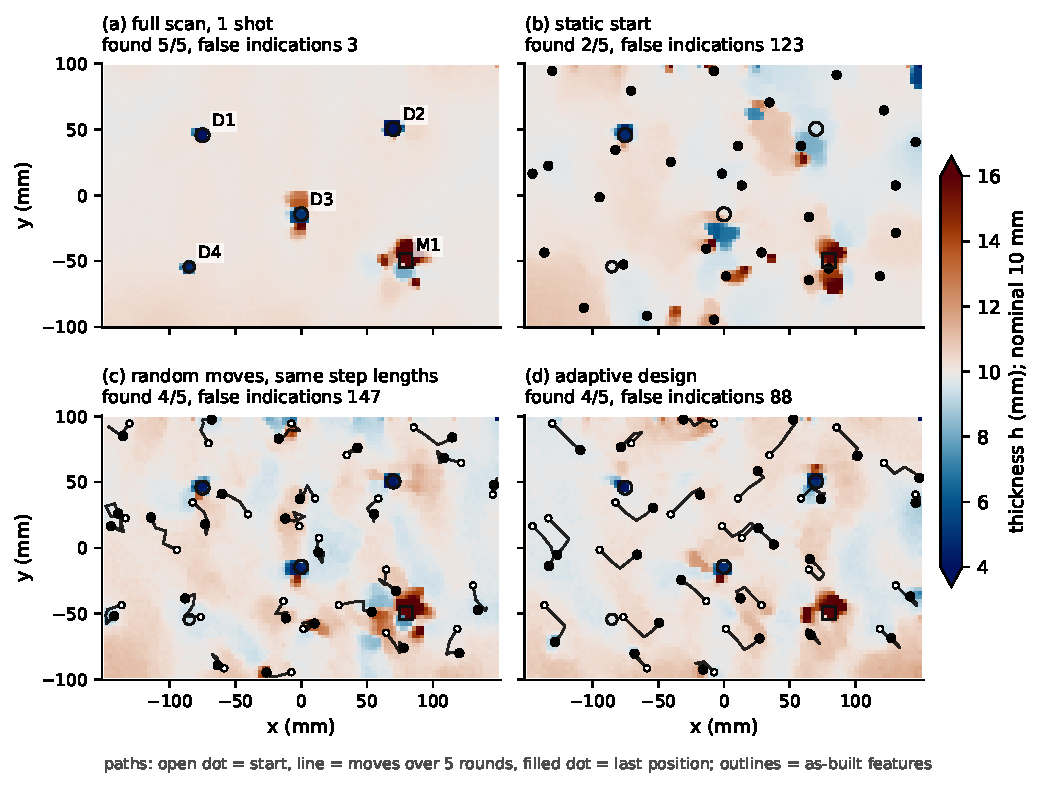
\includegraphics[width=0.9\linewidth]{F9_paths_a1_j30b.pdf}
\caption{\textbf{1 shot} (best adaptive run, j30b start): 4 of 5 found with 88 false indications, against 2 of 5 for the static start.}\label{fig:paths-1}
\end{figure}




\begin{figure}[ht]\centering
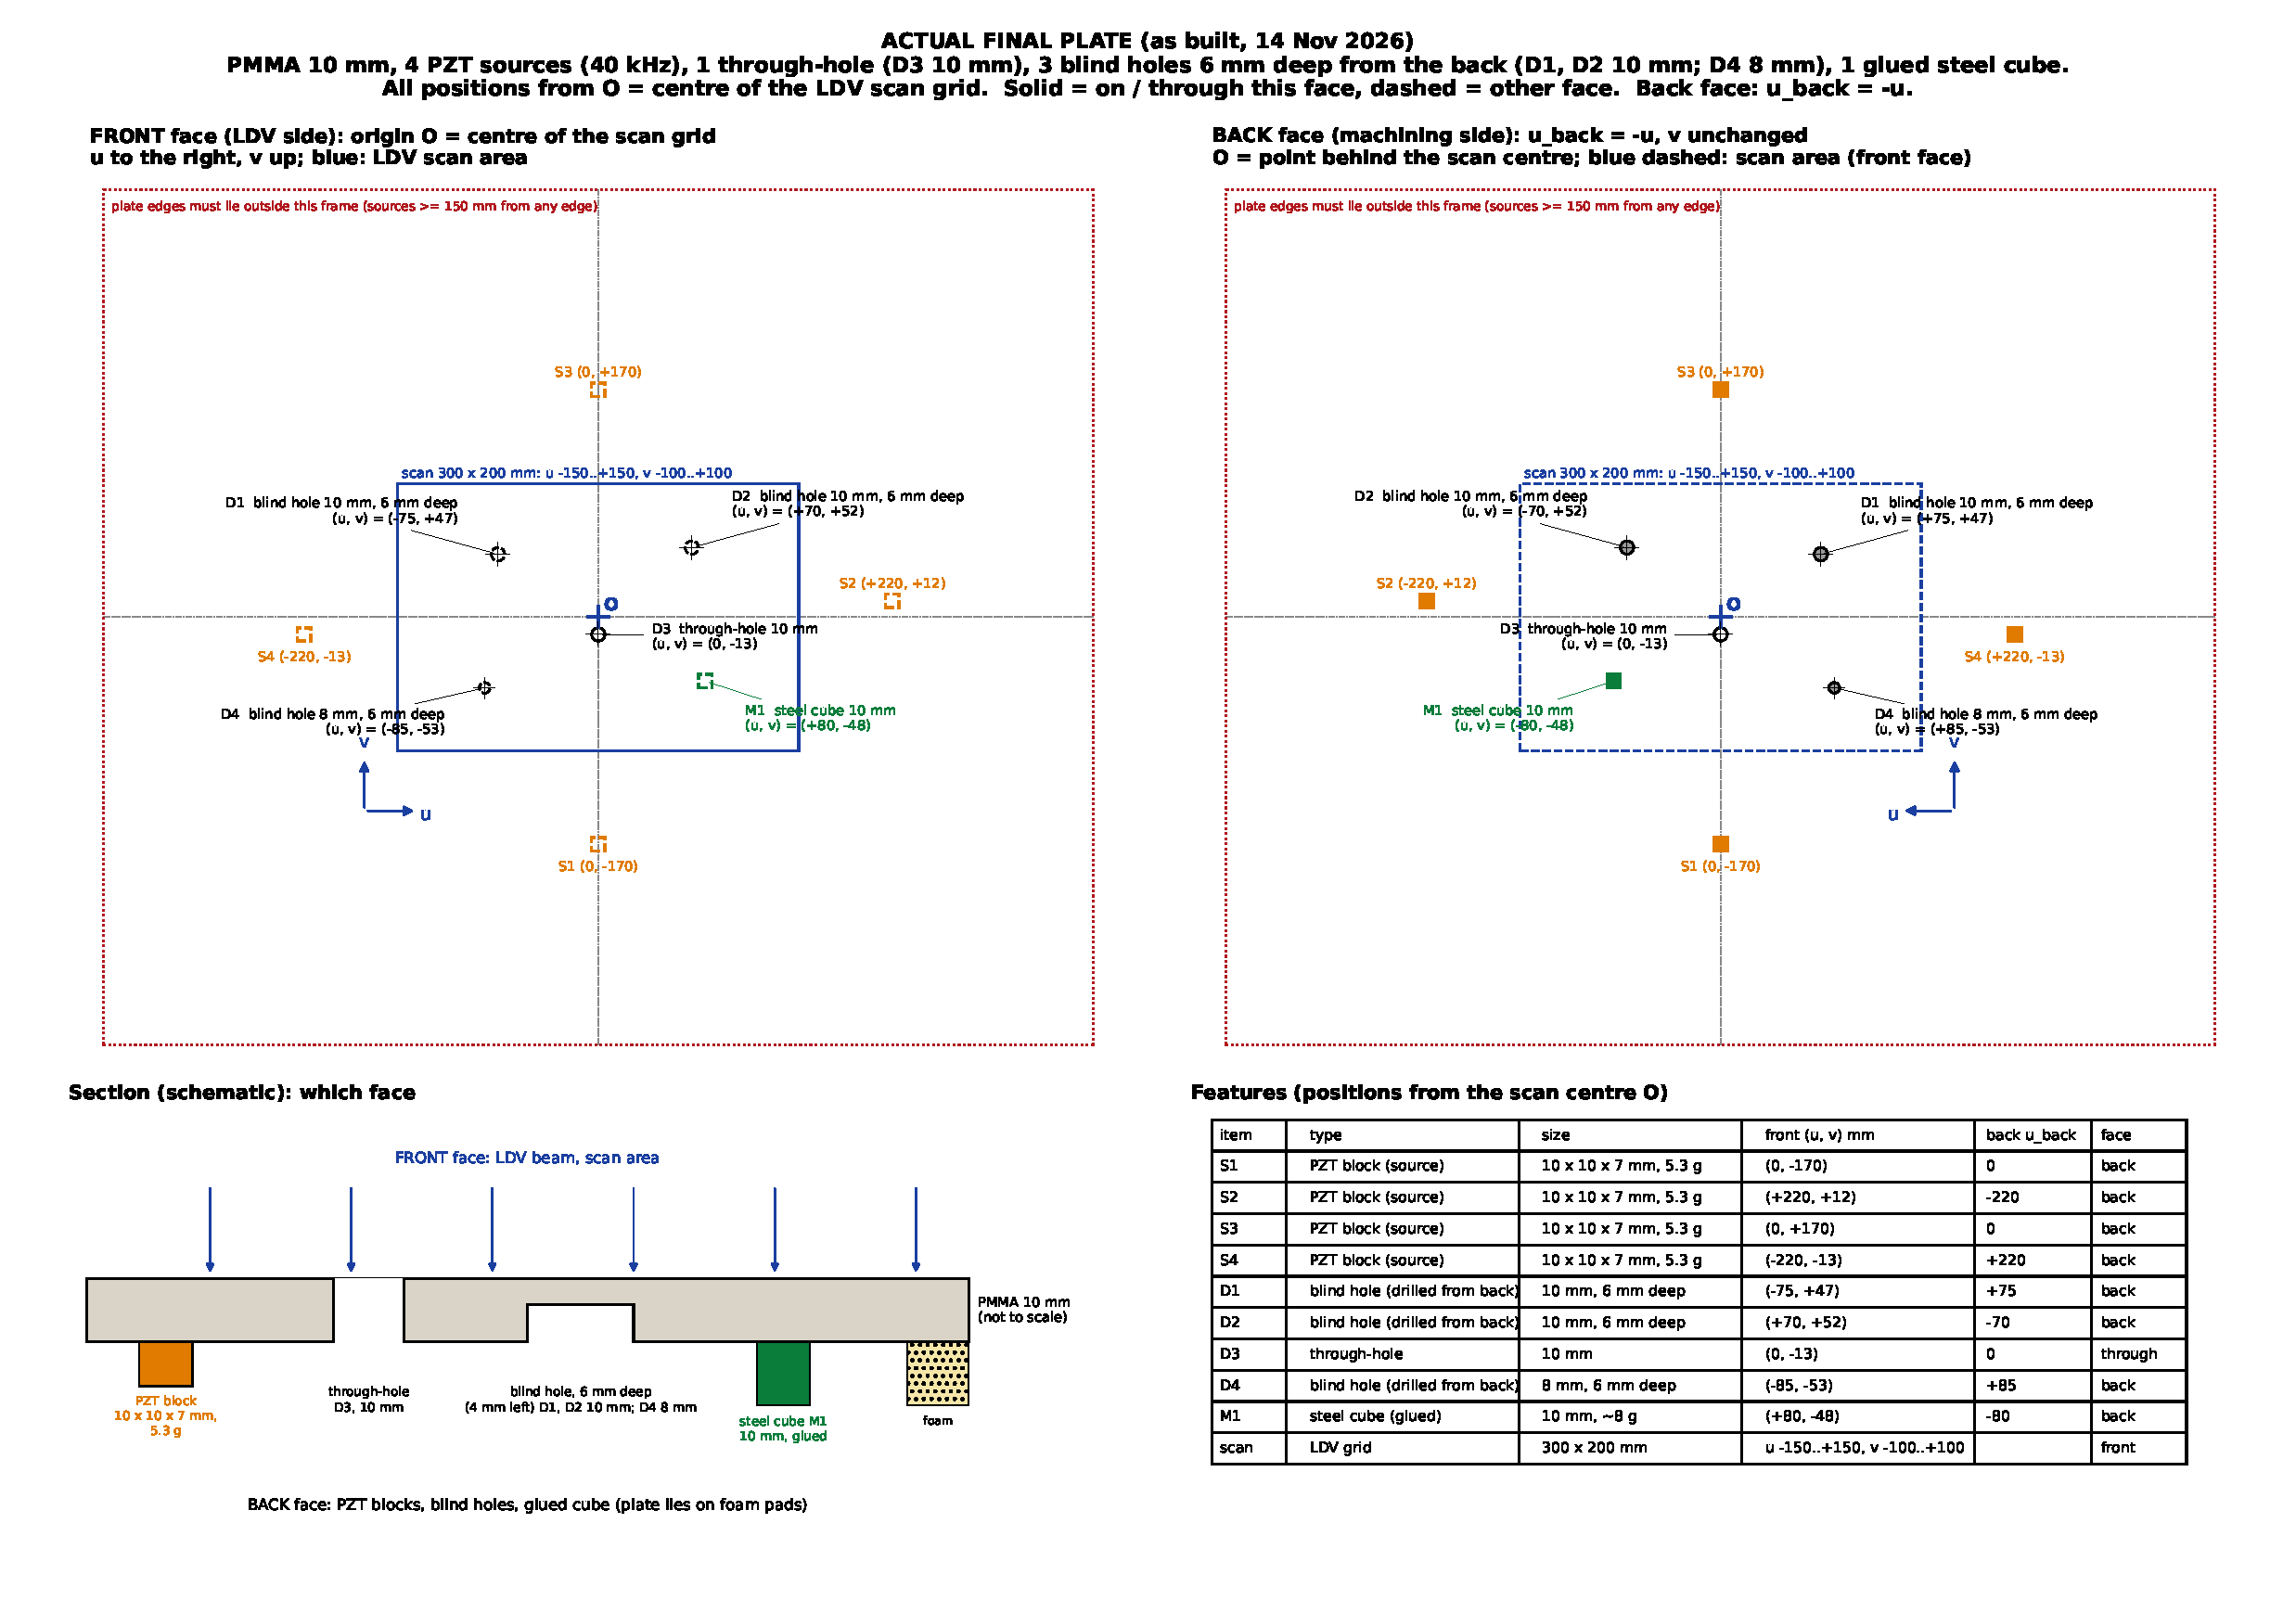
\includegraphics[width=\linewidth]{A1_specimen_full.pdf}
\caption{\textbf{Specimen drawing} (as built): front and back faces, section and coordinate table. PZT blocks 10$\times$10$\times$7\,mm, 5.3\,g.}\label{fig:drawing}
\end{figure}

\begin{figure}[ht]\centering
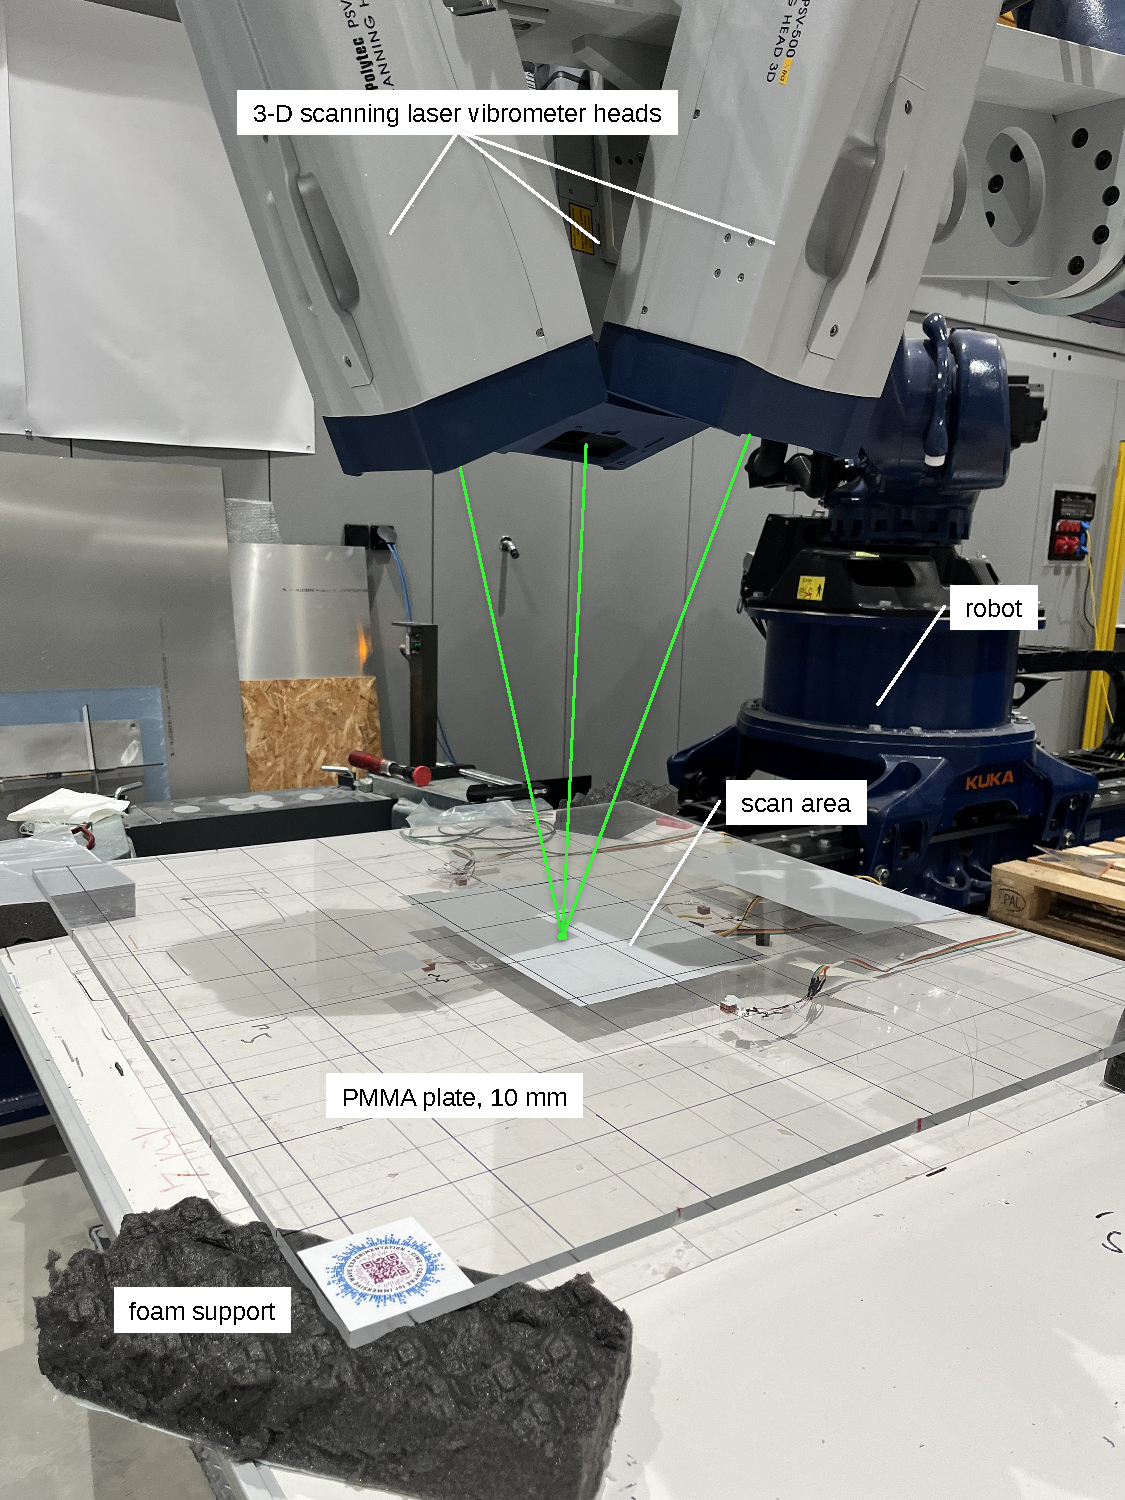
\includegraphics[width=0.5\linewidth]{A2_setup_edited.pdf}
\caption{\textbf{Laboratory setup}: 3-D scanning laser vibrometer on a robot above the PMMA plate (on foam supports); the white sheet marks the scan area; the three green beams converging on one scan point are drawn for illustration.}\label{fig:setup}
\end{figure}


\end{document}
